\subsection*{\large{Архитектура сервиса}}
\addcontentsline{toc}{subsection}{Архитектура сервиса}

Для решения задачи генерации векторных тайлов
для набора геоданных предлагается следующая архитектура.

\begin{figure}[H]
	\hspace*{-1 cm}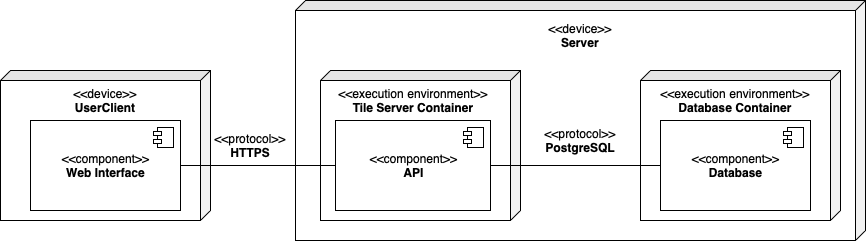
\includegraphics[width=\textwidth, left]{images/architecture/1}
	\caption{Диаграмма размещения}
	\label{pic:architecture__deployment-diagram}
\end{figure}
\vskip 5 mm

\noindent Компоненты представленные на диаграмме размещения (см. рис\ref{pic:architecture__deployment-diagram}):
\begin{itemize}
	\item \textbf{Web Interface} -- веб-интерфейс, позволяющий осуществлять взаимодействие с системой пользователю.
	\item \textbf{Tile Server Container}
	\begin{itemize}
		\item API -- веб-сервер, предоставляющий API для получения векторных тайлов.
	\end{itemize}
	\item \textbf{Database Container}
	\begin{itemize}
		\item Database -- база данных (БД), используемая для хранения данных генеральных планов.
	\end{itemize}
\end{itemize}


